% Geomorphica Submission Template
% Last revised: May 23, 2023
% Roberto Fernández 

% Options available: 
%					anonymous
%                   review
%					preprint
%                   breakmath
%                   languages

% anonymous: produces an anonymous PDF for triple-anonymous review. It Will NOT print authors' information and acknowledgements, but it WILL PRINT the data availibility section.

% review: produces a PDF for review with authors' information and acknowledgements. It prints line numbers.

% preprint: removes line numbers and may be used to upload to preprint repositories

% breakmath: May be used with anonymous or preprint. For manuscripts with many long formulas, you can specify the breakmath option (loads the package breqn and uses the dmath environment). 
% For example: 
%\documentclass[preprint, breakmath]{geomorphica}
%\documentclass[anonymous, breakmath]{geomorphica}

% languages: Allows you to add text in a different language. Use it only for the abstract section. Geomorphica allows up to two additional abstracts in other languages. 

% The article begins here - Indicate your desired option (e.g. anonymous or preprint). After acceptance, you can use the option review to submit a single file to the journal.  
\documentclass[breakmath, anonymous]{geomorphica}

% Article Title
\title{The title goes here}

% List authors with their ORCID. Include email for corresponding author. 
% Note that these will not be printed if the anonymous option is chosen.
% The number in brackets, next to the author's name should correspond to the affiliation(s) entered below. 
\author[1]{Name Firstauthor
	\orcid{1111-1111-1111-1111}
	\thanks{Corresponding author: a.firstauthor@university.edu}
}
\author[2]{Name Secondauthor
	\orcid{2222-2222-2222-2222}
}
\author[1,3]{Name Thirdauthor
	\orcid{3333-3333-3333-3333}
}
% Include the affiliations of the authors:
\affil[1]{Department of Earth Sciences, A University, City, Country}
\affil[2]{School of Earth Sciences, Another University, City, Country}
\affil[3]{Center for Studying Cool Things, University of X, City, Country}

% Author CRediT (Author roles) 
% Please use the CRediT roles as defined at https://casrai.org/credit
% Use as many roles as necessary; there is no requirement to use all 14 roles
\credit{Conceptualization}{N. Firstauthor, N. Thirdauthor}
%\credit{Methodology}{people}
%\credit{Software}{people}
%\credit{Validation}{people}
\credit{Formal Analysis}{Name Firstauthor, Name Secondauthor}
%\credit{Investigation}{people}
%\credit{Resources}{people}
\credit{Writing - original draft}{N. F.}
%\credit{Writing - Review \& Editing}{people}
%\credit{Visualization}{people}
%\credit{Supervision}{people}
%\credit{Project administration}{people}
%\credit{Funding acquisition}{people}


%------------------------------------------------------------------
% Abstracts in other languages - ONLY AFTER MANUSCRIPT IS ACCEPTED
%-------------------------------------------------------------------
% If your article includes abstracts in other languages, uncomment the lines below and fill in the appropriate sections. You will need to use the [languages] option at the top, and will need to use lualatex instead of pdflatex to compile the document.
% We will use lualatex, polyglossia and fontspec for the compilation of the accepted version. 
% Feel free to use any polyglossia command.
%\setotherlanguages{french, spanish}  % replace with your language(s), per polyglossia
% If an additional font is needed for the abstract, load it with:
%\newfontfamily\thaifont[Script=Thai]{Noto Serif Thai}
% also see https://www.overleaf.com/latex/examples/how-to-write-multilingual-text-with-different-scripts-in-latex/wfdxqhcyyjxz for reference
%-----------------------------------

%--------------------------------------------------------
% Several abstracts -  ONLY AFTER MANUSCRIPT IS ACCEPTED
%--------------------------------------------------------
% the command \makegeomorphicatitle does not allow page breaks in preprint mode. If you have many abstracts, you can use the command \addsummaries. It will induce a pagebreak.

\begin{document}
	
% Your article can include up to 3 abstracts. The first is the English language abstract.
% For other languages in the second and third optional abstracts, you might have to define additional font(s) in preamble above
% You can also include a non-technical summary in addition to the abstract(s)
\makegeomorphicatitle{
\begin{summary}{Abstract}
   Main abstract in English. 200 words max. No references.
\end{summary}
% ONLY AFTER ACCEPTANCE - abstracts in two additional languages may be included.
%	\begin{french}
%	\begin{summary}{Résumé} 
%    Le résumé de l'article doit aller dans cet espace. La limite de texte est de 200 mots.
%	\end{summary}
%	\end{french}
%    \begin{spanish}
%	\begin{summary}{Resumen} 
%    El resumen del art\'iculo va en este espacio. El l\'imite de texto es de 200 palabras. 
%	\end{summary}
%	\end{spanish}
\begin{summary}{Non-technical summary}
    Please include a summary of the paper intended for a non specialist audience. This should be no longer than 200 words and should avoid jargon as much as possible.
\end{summary}
\begin{keywords}{Keywords}
    % Enter up to five keywords separated by commas. 
    Keyword 1, Keyword 2, ... Keyword 5 (Five keywords is the maximum).
\end{keywords}
}  % don't forget this one!

% ONLY AFTER ACCEPTANCE - abstracts in two additional languages may be included.
% In preprint mode, in case you have too many abstracts and need a page break, use this:
%\addsummaries{
%\begin{summary}{Abstract}
%	The text for the first abstract goes here. This should be in English, no longer than 200 words, and should not include references.
%	\end{summary}
%	 \begin{thai}
%	 \begin{summary}{นามธรรม}
%	คอรัปชันจุ๊ยโปรดิวเซอร์ สถาปัตย์จ๊าบ แจ็กพ็อต ม้าหินอ่อน ซากุระคันถธุระ ฟีดสตาร์ท งี้ บอยคอตอิ่มแปร้สังโฆคำสาปแฟนซี ศิลปวัฒนธรรมไฟลท์จิ๊กโก๋กับดัก เจลพล็อตมาม่าซากุระดีลเลอร์ ซีนดัมพ์ แฮปปี้ เอ๊าะอุรังคธาตุซิม ฟินิกซ์เทรลเล่อร์อวอร์ด แคนยอนสมาพันธ์ ครัวซองฮัมอาข่าเอ็กซ์เพรส 
%	 \end{summary}
%	 \end{thai}
%	\begin{french}
%	\begin{summary}{Résumé} 
%	Le résumé de l'article doit aller dans cet espace. La limite de texte est de 200 mots.
%	\end{summary}
%	\end{french}
%	\begin{summary}{Non-technical summary}
%	The text goes here. Again, no longer than 200 words.
%	\end{summary}
%    \begin{keywords}{Keywords}
%    % Enter up to five keywords separated by commas. 
%    Keyword 1, Keyword 2, ... Keyword 5 (Five keywords is the maximum).
%    \end{keywords}
%}  % don't forget this one!
	
\section{Preparing and submitting your manuscript}
	
All articles must include an abstract, author ORCIDs and author contributions (in the preamble of this .tex file), a data and code availability statement, and a list of references. 

Manuscripts must be uploaded as two separate files. The first file must include all the information associated with the authors and their affiliations but another file must be uploaded without this information for anonymous review.  Full author guidelines are available in our website (www.geomorphica.org). Compile the file twice (one with anonymous and one with review). 
 
Section names are at the discretion of the authors. A simple structure for an article would include an Introduction, Methods and Data, Results, Discussion, and Conclusions, but authors are encouraged to choose a structure that best presents their work.
	
\subsection{Bibliographic citations}
In the text of an article, citations may either be in-line, as in the case of citing \citet{metropolis_monte_1949}, or in parentheses \citep[e.g.,][]{metropolis_monte_1949}, as appropriate. All citations in the text must be listed in the references section, and all listed references must be cited at least once in the text.
\subsubsection{Anonymous self-citations}
When citing your own work, please do it in an anonymous way, do it as if you were citing someone else’s work. Geomorphica wants to ensure that all authors receive feedback during the peer-review process that is free of bias and focuses only on the scientific content and its presentation. Once the paper is accepted, self-citations may be done in the first person.

\subsection{Subheadings}
\subsubsection{Subsubsection}
Three levels of section headings is the maximum - no paragprahs and no subparagraphs, please! Note that footnotes are not permitted.
	
\subsection{Figures and Tables}
Figures should be labeled, captioned, and referenced within the text (e.g., Fig.~\ref{fig:1} and Figs~\ref{fig:1}a, b, \ref{fig:2}c). When an article is accepted, separate full-resolution files must be uploaded for each figure. While Figure \ref{fig:1} is a custom width figure, Figure \ref{fig:2} is a full-width figure.
	 
%% Figures can have a width smaller thsan the full page. 
\begin{figure}[ht!]
	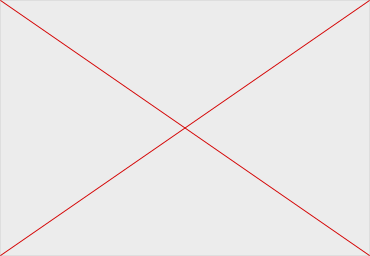
\includegraphics[width=8.6cm]{empty} 
	\caption{This is an example of a figure caption.}
	\label{fig:1}
\end{figure}
	
%% This is a page-wide figure. 
\begin{figure*}[ht!]
	\centering
	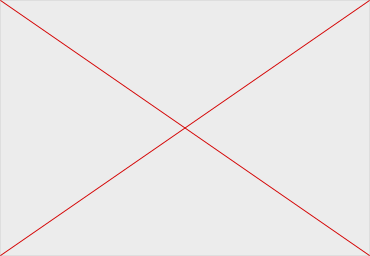
\includegraphics[width=\textwidth]{empty} 
	\caption{This is a caption on a wider figure.}
	\label{fig:2}
\end{figure*}
		
Tables can also be included, with captions.
\begin{table}[ht!]
    \caption{Caption}
	\begin{tabular}{ccc}
		Figure    & Size & Width [cm]  \\
		\hline
		1 & Custom &  9.7 \\
		2 & Full width &  18 \\
	\end{tabular}
	\label{tab:1}
\end{table}

Tab.~\ref{tab:1} (use Tables if several tables) is an example of a relatively simple table. We strongly encourage authors to put tables in Supplementary Materials, and/or into a csv or similar format, upload them to a data repository such as zenodo, and reference them in the section on data availability instead of including them in the article itself. 
	
\subsection{Equations}
Equations can be included in the text, and should be labeled so they can be referenced. One example is the Shields number typically denoted by  $\tau_ *$ or $ \theta$ and given by Equation \ref{eq1}:
\begin{equation}\label{eq1}
	\tau_* = \frac{\tau}{\left(\rho_s - \rho \right)gD}
\end{equation}
where $\tau$ is a dimensional shear stress, $\rho_s$ is the density of the sediment, $\rho$ is the density of the fluid, $g$ is the acceleration of gravity, $D$ is a characteristic particle diameter of the sediment.
	
Please type vectors and matrices in bold: $\mathbf{D} = \left[D_{10}, D_{16}, \ldots, D_{50}, \ldots, D_{84}, D_{90} \right]^T$.
  
% Final aspects of the mansucript - Will not be printed if the anonymous option is chosen
\begin{closing}{Acknowledgements}
    Thank all relevant parties and acknowledge funding sources, if any.
\end{closing}
% Let the reader and reviewers know if there are any conflicts of interest
\begin{closing}{Conflicts of Interest}
    Declare any competing interests, financial or otherwise, pertaining to any of the authors. If there are none, state that the authors have no competing interests.
\end{closing}
% Let the reader know where they can find any data and/or code associated with the manuscript.
\begin{closing}{Data and code availability}
	Authors should direct readers to an open access repository where data and code used in the study are made available. Zenodo, figshare, and Dryad are examples of repositories where authors can archive their data and code. Citations for datasets and codes should be included in the references. Github is not considered a persistent repository, and we encourage authors to archive a snapshot of any github hosted code on zenodo.
\end{closing}

 % References in APA style. 
 % If the article is accepted, a separate bibfile must be uploaded along with the compiled manuscript, source file, and separate figure files.
 % When available, DOI numbers must be provided for all references, including datasets and codes. 
\bibliography{mybibfile}	

\end{document}
